\documentclass[14pt]{extbook}
\usepackage{multicol, enumerate, enumitem, hyperref, color, soul, setspace, parskip, fancyhdr} %General Packages
\usepackage{amssymb, amsthm, amsmath, bbm, latexsym, units, mathtools} %Math Packages
\everymath{\displaystyle} %All math in Display Style
% Packages with additional options
\usepackage[headsep=0.5cm,headheight=12pt, left=1 in,right= 1 in,top= 1 in,bottom= 1 in]{geometry}
\usepackage[usenames,dvipsnames]{xcolor}
\usepackage{dashrule}  % Package to use the command below to create lines between items
\newcommand{\litem}[1]{\item#1\hspace*{-1cm}\rule{\textwidth}{0.4pt}}
\pagestyle{fancy}
\lhead{Module6}
\chead{}
\rhead{Version B}
\lfoot{9356-6875}
\cfoot{}
\rfoot{testing}
\begin{document}

\begin{enumerate}
\litem{
Describe the end behavior of the polynomial below.\[ f(x) = -9(x - 4)^{3}(x + 4)^{8}(x + 9)^{3}(x - 9)^{3} \]\begin{enumerate}[label=\Alph*.]
\begin{multicols}{2}\item 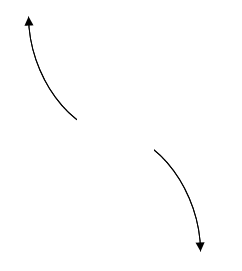
\includegraphics[width = 0.3\textwidth]{../Figures/polyEndBehaviorAB.png}\item 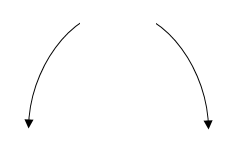
\includegraphics[width = 0.3\textwidth]{../Figures/polyEndBehaviorBB.png}\item 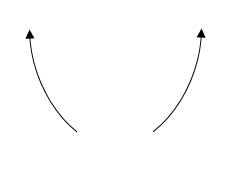
\includegraphics[width = 0.3\textwidth]{../Figures/polyEndBehaviorCB.png}\item 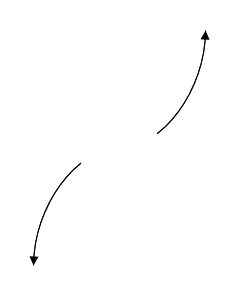
\includegraphics[width = 0.3\textwidth]{../Figures/polyEndBehaviorDB.png}\end{multicols}\item None of the above.
\end{enumerate} }
\litem{
Which of the following equations \textit{could} be of the graph presented below?
\begin{center}
    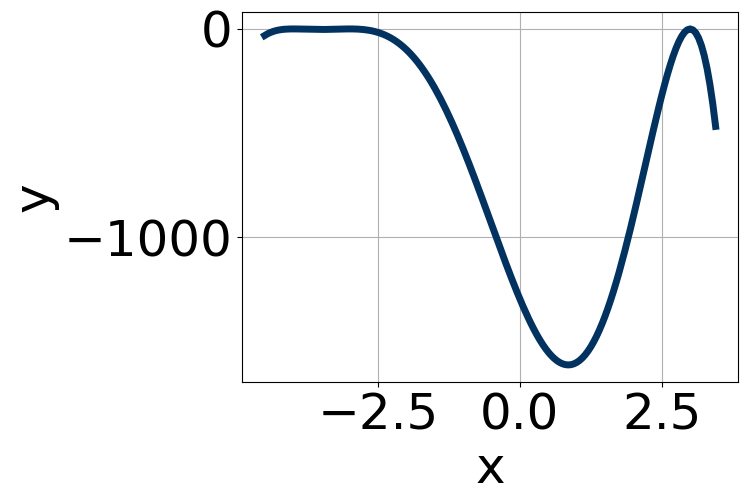
\includegraphics[width=0.5\textwidth]{../Figures/polyGraphToFunctionB.png}
\end{center}
\begin{enumerate}[label=\Alph*.]
\item \( -14(x + 1)^{5} (x - 3)^{11} (x - 1)^{9} \)
\item \( 20(x + 1)^{6} (x - 3)^{10} (x - 1)^{5} \)
\item \( 12(x + 1)^{4} (x - 3)^{5} (x - 1)^{9} \)
\item \( -11(x + 1)^{10} (x - 3)^{5} (x - 1)^{7} \)
\item \( 6(x + 1)^{11} (x - 3)^{11} (x - 1)^{9} \)

\end{enumerate} }
\litem{
Construct the lowest-degree polynomial given the zeros below. Then, choose the intervals that contain the coefficients of the polynomial in the form $ax^3+bx^2+cx+d$.\[ \frac{3}{5}, -5, \text{ and } -7 \]\begin{enumerate}[label=\Alph*.]
\item \( a \in [3, 17], b \in [-61, -55], c \in [131, 141], \text{ and } d \in [104, 111] \)
\item \( a \in [3, 17], b \in [62, 68], c \in [208, 220], \text{ and } d \in [104, 111] \)
\item \( a \in [3, 17], b \in [56, 59], c \in [131, 141], \text{ and } d \in [104, 111] \)
\item \( a \in [3, 17], b \in [4, 14], c \in [-173, -167], \text{ and } d \in [-106, -101] \)
\item \( a \in [3, 17], b \in [56, 59], c \in [131, 141], \text{ and } d \in [-106, -101] \)

\end{enumerate} }
\litem{
Construct the lowest-degree polynomial given the zeros below. Then, choose the intervals that contain the coefficients of the polynomial in the form $x^3+bx^2+cx+d$.\[ 4 + 3 i \text{ and } -4 \]\begin{enumerate}[label=\Alph*.]
\item \( b \in [0.1, 1.1], c \in [-0.68, 0.29], \text{ and } d \in [-17.9, -15.3] \)
\item \( b \in [3, 6.4], c \in [-7.36, -6.73], \text{ and } d \in [-101.4, -98.9] \)
\item \( b \in [0.1, 1.1], c \in [0.54, 2.17], \text{ and } d \in [-13.2, -10.4] \)
\item \( b \in [-5, -2.6], c \in [-7.36, -6.73], \text{ and } d \in [98.6, 102.8] \)
\item \( \text{None of the above.} \)

\end{enumerate} }
\litem{
Construct the lowest-degree polynomial given the zeros below. Then, choose the intervals that contain the coefficients of the polynomial in the form $ax^3+bx^2+cx+d$.\[ \frac{-4}{3}, -2, \text{ and } \frac{3}{2} \]\begin{enumerate}[label=\Alph*.]
\item \( a \in [6, 11], b \in [-7, -3], c \in [-23, -21], \text{ and } d \in [23, 25] \)
\item \( a \in [6, 11], b \in [-15, -9], c \in [-14, -11], \text{ and } d \in [23, 25] \)
\item \( a \in [6, 11], b \in [8, 16], c \in [-14, -11], \text{ and } d \in [-31, -20] \)
\item \( a \in [6, 11], b \in [-35, -27], c \in [46, 47], \text{ and } d \in [-31, -20] \)
\item \( a \in [6, 11], b \in [8, 16], c \in [-14, -11], \text{ and } d \in [23, 25] \)

\end{enumerate} }
\litem{
Construct the lowest-degree polynomial given the zeros below. Then, choose the intervals that contain the coefficients of the polynomial in the form $x^3+bx^2+cx+d$.\[ -5 + 4 i \text{ and } -3 \]\begin{enumerate}[label=\Alph*.]
\item \( b \in [12, 15], c \in [60, 72], \text{ and } d \in [122, 124] \)
\item \( b \in [-6, 3], c \in [-9, 0], \text{ and } d \in [-15, -4] \)
\item \( b \in [-18, -8], c \in [60, 72], \text{ and } d \in [-124, -121] \)
\item \( b \in [-6, 3], c \in [6, 14], \text{ and } d \in [6, 19] \)
\item \( \text{None of the above.} \)

\end{enumerate} }
\litem{
Describe the end behavior of the polynomial below.\[ f(x) = -8(x - 2)^{4}(x + 2)^{7}(x + 8)^{2}(x - 8)^{3} \]\begin{enumerate}[label=\Alph*.]
\begin{multicols}{2}\item 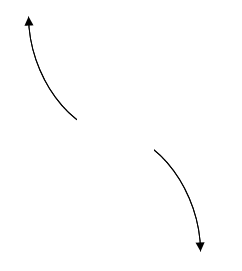
\includegraphics[width = 0.3\textwidth]{../Figures/polyEndBehaviorCopyAB.png}\item 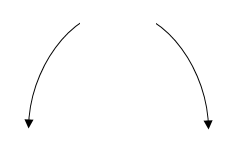
\includegraphics[width = 0.3\textwidth]{../Figures/polyEndBehaviorCopyBB.png}\item 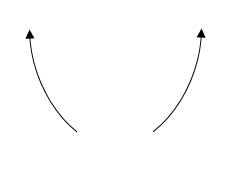
\includegraphics[width = 0.3\textwidth]{../Figures/polyEndBehaviorCopyCB.png}\item 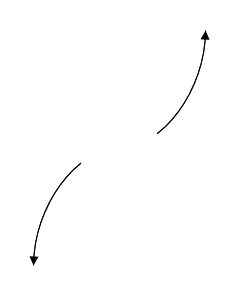
\includegraphics[width = 0.3\textwidth]{../Figures/polyEndBehaviorCopyDB.png}\end{multicols}\item None of the above.
\end{enumerate} }
\litem{
Describe the zero behavior of the zero $x = -8$ of the polynomial below.\[ f(x) = 6(x - 2)^{4}(x + 2)^{3}(x + 8)^{6}(x - 8)^{3} \]\begin{enumerate}[label=\Alph*.]
\begin{multicols}{2}\item 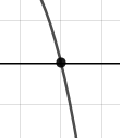
\includegraphics[width = 0.3\textwidth]{../Figures/polyZeroBehaviorAB.png}\item 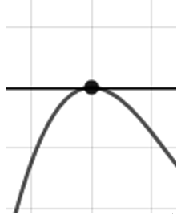
\includegraphics[width = 0.3\textwidth]{../Figures/polyZeroBehaviorBB.png}\item 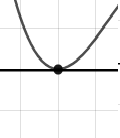
\includegraphics[width = 0.3\textwidth]{../Figures/polyZeroBehaviorCB.png}\item 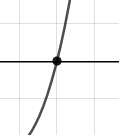
\includegraphics[width = 0.3\textwidth]{../Figures/polyZeroBehaviorDB.png}\end{multicols}\item None of the above.
\end{enumerate} }
\litem{
Describe the zero behavior of the zero $x = -9$ of the polynomial below.\[ f(x) = 3(x + 9)^{8}(x - 9)^{9}(x - 4)^{3}(x + 4)^{7} \]\begin{enumerate}[label=\Alph*.]
\begin{multicols}{2}\item 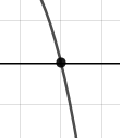
\includegraphics[width = 0.3\textwidth]{../Figures/polyZeroBehaviorCopyAB.png}\item 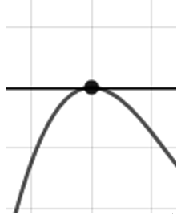
\includegraphics[width = 0.3\textwidth]{../Figures/polyZeroBehaviorCopyBB.png}\item 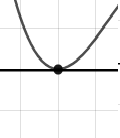
\includegraphics[width = 0.3\textwidth]{../Figures/polyZeroBehaviorCopyCB.png}\item 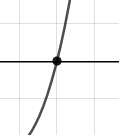
\includegraphics[width = 0.3\textwidth]{../Figures/polyZeroBehaviorCopyDB.png}\end{multicols}\item None of the above.
\end{enumerate} }
\litem{
Which of the following equations \textit{could} be of the graph presented below?
\begin{center}
    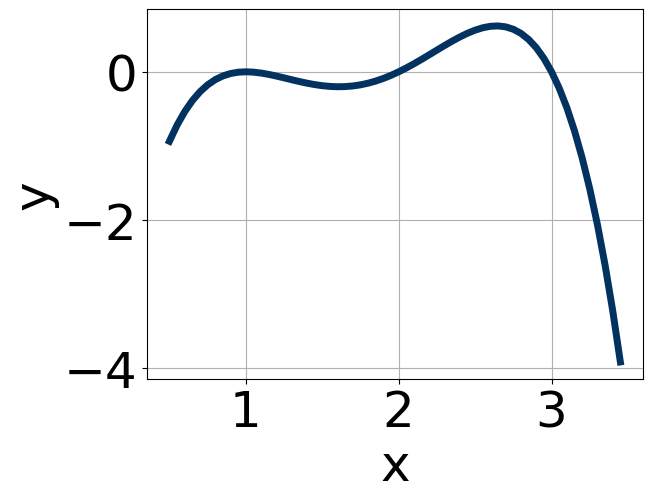
\includegraphics[width=0.5\textwidth]{../Figures/polyGraphToFunctionCopyB.png}
\end{center}
\begin{enumerate}[label=\Alph*.]
\item \( 13(x - 1)^{11} (x + 1)^{11} (x - 2)^{5} \)
\item \( 14(x - 1)^{4} (x + 1)^{9} (x - 2)^{9} \)
\item \( -10(x - 1)^{5} (x + 1)^{9} (x - 2)^{11} \)
\item \( -19(x - 1)^{10} (x + 1)^{9} (x - 2)^{9} \)
\item \( 9(x - 1)^{4} (x + 1)^{8} (x - 2)^{11} \)

\end{enumerate} }
\end{enumerate}

\end{document}